\section{Policy Gradients}
Policy gradient algorithms directly optimize the policy $\pi_\theta(\cdot \mid  s)$. The goal is to maximize the expected return under $\pi_\theta$:
\[
    \max_\theta J(\theta) = \E_{\tau \sim \pi_\theta} [R(\tau)]
\]
Using the log-derivative trick ($\nabla f = f \nabla \log f$) and the likelihood of a trajectory $\tau$:
\[
    \pi_\theta(\tau) = \rho_0(s_0) \prod_{t=0}^T P(s_{t+1} \mid  s_t, a_t) \pi_\theta(a_t \mid  s_t)
\]
the \emph{policy gradient} can be derived:
\begin{align}
    \nabla_\theta J(\theta) 
    &= \E_{\tau \sim \pi_\theta} [\nabla_\theta \log \pi_\theta(\tau) R(\tau)] \nonumber \\
    &= \E_{\tau \sim \pi_\theta} \left[\sum_{t=0}^T R(\tau) \nabla_\theta \log \pi_\theta(a_t \mid  s_t) \right]
    \label{eq:policy-gradient}
\end{align}


Learning the optimal policy can be easier than learning all the action values $Q(s,a)$, and directly optimizing $\pi_\theta$ makes it possible to have smoother updates and more stable convergence than Q-learning. In addition, all policy gradient algorithms work with continuous/infinite action spaces, and can encourage exploration with additional rewards (entropy). However, they can be less adapted to tabular environments and are often less sample-efficient than value-based approaches, which typically use memory buffers.

\subsection{On-Policy}
\paragraph{REINFORCE}
Based on eq. \ref{eq:policy-gradient}, the REINFORCE algorithm simply uses a Monte-Carlo estimate of $\nabla_\theta J(\theta)$ to optimize $\pi_\theta$, and increase the likelihood of trajectories with high rewards.

\begin{algorithm}[H]
\DontPrintSemicolon
\For{a number of epochs}{
    \While{not enough samples}{
        collect trajectory $\tau_i=(s_0^i, a_0^i, \dots, s_{T_i}^i)$ by running active policy $\pi_\theta$
    }
    $\hat{g} \leftarrow \sum_i \sum_t R(\tau^i) \nabla_\theta \log \pi_\theta(a_t^i \mid  s_t^i)$ \tcp*{compute policy gradient estimate}
    $\theta \leftarrow \theta + \alpha \hat{g}$ \;
}
\caption{Vanilla REINFORCE}
\label{algo:reinforce}
\end{algorithm}

It is unbiased but typically has very high variance and is slow to converge. Variance can be reduced using alternatives expressions of the gradient (all three can be combined):
\begin{itemize}
    \item \emph{Causality (don't let the past distract you)}
    Intuitively, rewards obtained before taking an action do not bring any information, they are just noise. Indeed $R(\tau)$ can be replaced by the \emph{reward-to-go} $R_t(\tau) = \sum_{t'=t}^T r_t'$ without making the policy gradient expression biased \demo.
    \item \emph{Baseline}
    For any function $b:\mathcal{S} \rightarrow \mathbb{R}$, we have:
    \[
        \E_{\tau \sim \pi_\theta} \left[\sum_{t=0}^T b(s_t) \nabla_\theta \log \pi_\theta(a_t \mid  s_t) \right] = 0
    \]
    Hence \demo we can use $(R(\tau) - b(s_t))$ instead of $R(\tau)$, and the variance is minimal when choosing $b(s) = V^\pi(s)$  (e.g. by fitting $b(s_t)$ to  $R_t(\tau)$).
    \item \emph{Discount}
    Using a discounted return $R(\tau) = \sum_{t=0}^T \gamma r_t$ can also reduce the variance but, unlike the 2 previous techniques, it makes the gradient biased. 
\end{itemize}

More generally, the policy gradient can be expressed as:
\begin{equation}
    \nabla_\theta J(\theta) 
    = \E_{\tau \sim \pi_\theta} \left[\sum_{t=0}^T \Psi_t \nabla_\theta \log \pi_\theta(a_t \mid  s_t) \right]
    \label{eq:policy-gradient2}
\end{equation}

Where $\Psi_t$ may be the reward $R(\tau)$, the reward-to-go $R_t(\tau)$, with or without a baseline (e.g. $R_t(\tau) - b(s_t)$).

\paragraph{Actor-Critic}
The policy gradient (eq. \ref{eq:policy-gradient2}) can also be expressed \demo with:
\begin{itemize}
    \item $\Psi_t = Q^\pi(s_t,a_t)$: state-action value function
    \item $\Psi_t = A^\pi(s_t,a_t)$: advantage function
    \item $\Psi_t = r_t + \gamma V^\pi(s_{t+1}) - V^\pi(s_t) = \delta_t$: TD error
\end{itemize}
Actor-critic methods combine the strengths of policy gradient and value-based methods by estimating a critic ($Q^\pi$, $V^\pi$ and/or $A^\pi$) in order to better optimize the actor (policy $\pi_\theta$). Adding a critic reduces the variance, but estimation errors introduce a bias as soon as the critic is not perfect.

\paragraph{Actor-Critic with compatible functions}
We can try to approximate $A^\pi$ with a function $f_\phi: \mathcal{S} \times \mathcal{A} \rightarrow \mathbb{R}$. According to the \emph{Compatible Function Approximation Theorem} \cite{sutton2000policy} \demo, if $f_\phi$ satisfies
\begin{equation}
    \forall s, a, \nabla_\phi f_\phi(s,a) = \nabla_\theta \log \pi_\theta(a\mid s)
    \qquad \text{(i.e. $f_\phi$ is \emph{compatible})}
\label{eq:compat-fct-1}
\end{equation}
\begin{equation}
    \E_{\tau \sim \pi_\theta} \left[ \sum_{t=0}^T \gamma^t (Q^\pi(s_t,a_t) - f_\phi(s_t,a_t)) \nabla_\theta \log \pi_\theta(a_t\mid s_t)\right] = 0
\label{eq:compat-fct-2}
\end{equation}
then the policy gradient is exact:
\[
    \nabla_\theta J(\theta) 
    = \E_{\tau \sim \pi_\theta} \left[\sum_{t=0}^T \gamma^t f_\phi(s_t,a_t) \nabla_\theta \log \pi_\theta(a_t \mid  s_t) \right]
\]
Eq. \ref{eq:compat-fct-1} can be satisfied with $f_\phi(s,a) = \nabla_\theta \log \pi_\theta(s,a)^T \phi$, and eq. \ref{eq:compat-fct-2} by solving:
\[
    \min_{\phi, w} \E_{s, a \sim \pi_\theta}\left[
    \left(Q^\pi(s,a) - f_\phi(s,a) - v_w(s)\right)^2
    \right]
\]
for some function $v_w:\mathcal{S} \rightarrow \mathbb{R}$ \demo. In practice, TD is used to estimate $V^\pi$ with $v_w$, and $Q^\pi$ with $f_\phi + v_w$, so that $f_\phi(s,a) \approx A^\pi(s,a)$.

\paragraph{Actor-Critic with Generalized Advantage Estimation (GAE) \cite{schulman2015high}}
This method only requires estimating $V^\pi$ (easier to learn than $Q^\pi(s,a) \forall s,a$, especially in high dimension) to obtain an estimate of $A^\pi$.
Similar to multi-steps learning, we can define the \emph{n-steps advantage estimate}:
\begin{equation}
    A_t^{(n)} = r_t + \gamma r_{t+1} + \dots + \gamma^{n-1} r_{t+n-1} + \gamma^n V^\pi(s_{t+n}) - V^\pi(s_t)
\label{eq:n-steps-advantage}
\end{equation}
and control the bias-variance trade-off with $n$ ($n=1$: lower variance but higher bias when the estimate of $V^\pi$ is wrong, $n\rightarrow \infty$: Monte-Carlo estimate, no bias but higher variance). Like TD($\lambda$) learning, GAE averages the estimates and uses $\lambda \in [0,1]$ to control the trade-off:
\[
    A_t^{GAE(\gamma,\lambda)} = (1-\lambda) \sum_{n=0}^\infty \lambda^n A_t^{(n)} = \sum_{n=0}^\infty (\lambda \gamma)^n \delta_{t+n}
\]
Here as well, eligibility traces are a way to implement GAE$(\gamma,\lambda)$. Indeed, we can re-write the sample estimate of the policy gradient:
\[
    \sum_{t=0}^\infty A_t^{GAE(\gamma,\lambda)} \nabla_\theta \log \pi_\theta(a_t \mid  s_t)
    = \sum_{t=0}^\infty \nabla_\theta \log \pi_\theta(a_t \mid  s_t) \sum_{n=0}^\infty (\gamma \lambda)^n \delta_{t+n}
\]

\begin{algorithm}[H]
\DontPrintSemicolon
\For{a number of episodes}{
    initialize $s_0$ and set $e_0(s)=0, \forall s$\;
     \While{episode not done}{
        take action $a_t \sim \pi(\cdot \mid s_t)$, observe $r_t$ and $s_{t+1}$ \;
        \For{all $s$}{
          $e_t(s) \leftarrow \lambda \gamma e_{t-1}(s) + \mathbbm{1}_{s_t=s}$ \tcp*{this leads to $e_t(s) = \sum_{k=0}^t(\lambda \gamma)^{t-k} \mathbbm{1}_{s_k=s}$}
          $V(s_t) \leftarrow V(s_t) + \alpha e_t(s) \delta_t$ \;
        } 
    }
}
\caption{Actor-critic with GAE, using eligibility traces}
\label{algo:gae-eligibility-traces}
\end{algorithm}

% todo: add algos, e.g. learn $V^\pi ?$

\paragraph{A2C / A3C}
\emph{Asynchronous Advantage Actor Critic} (A3C) \cite{mnih2016asynchronous} and its synchronous version A2C are two widely used actor-critic methods. They both run $n$ environments in parallel to get better estimates of the returns (more samples = less variance).
\begin{itemize}
    \item Both a policy $\pi_\theta$ and a value function $V^{\pi}_{\theta_v}$ are learned. Most of the layers are shared (fig. \ref{fig:actor-critic-architecture}).
    \item \emph{Asynchronous}. The A3C updates are done asynchronously: each agent sends its gradient to the global network every $k$ steps and updates its local weights after that.
    \item \emph{Advantage}. Use the $n$-steps return (forward view, eq. \ref{eq:n-steps-advantage}) to learn $V^\pi_{\theta_v}$ and to estimate the advantage function $A^\pi$.
\end{itemize}
The A2C algorithm works the same way but with synchronous, deterministic updates. It waits for all agents to be done with the $k$ steps, before performing a batch update and updating all weights at the same time.

% todo: give actual formula (and algo) of A3C/A2C, cf https://arxiv.org/pdf/1611.01224.pdf
\begin{figure}[H]
    \centering
    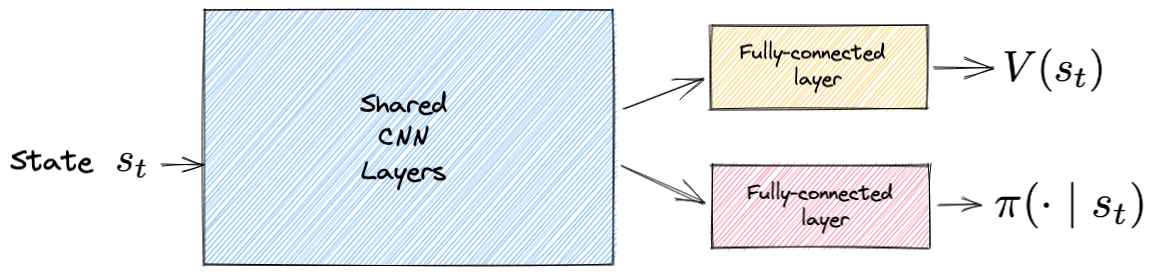
\includegraphics[width=0.8\linewidth]{figures/shared-actor-critic-network.png}
    \caption{Example of a shared network architecture for actor-critic methods.}
    \label{fig:actor-critic-architecture}
\end{figure}

\paragraph{Entropy}
To encourage exploration and avoid converging on a deterministic policy too fast, an entropy cost can be added to the policy gradient update: 
\[
    \theta \leftarrow \theta + \alpha (\nabla_\theta J(\theta) + \nabla_\theta H_\theta(s_t))
\]
With
\[
    H_\theta(s_t) = - \sum_a \pi_\theta(a_t\mid s_t) \log \pi_\theta(a_t\mid s_t)
\]
the entropy term to maximize.

\paragraph{Relative Policy Performance Bound}
Instead of looking directly for $\max_\pi J(\pi)$, we can optimize the \emph{relative performance} between $\pi$ and and arbitrary policy $\pi_{old}$: $\max_\pi J(\pi) - J(\pi_{old})$. For any policies $\pi = \pi_\theta$, $\pi_{old} = \pi_{\theta_{old}}$, we have the \emph{relative performance bound}:
\begin{align}
    J(\pi) - J(\pi_{old}) 
    &= \E_{\tau \sim \pi} \left[ \sum_{t=0}^\infty \gamma^t A^{\pi_{old}}(s_t,a_t) \right] \nonumber\\
    &= \frac{1}{1-\gamma} \E_{s\sim d^\pi(s), a \sim \pi_{old}(a\mid s)} \left[ \frac{\pi(a\mid s)}{\pi_{old}(a\mid s)} A^{\pi_{old}}(s,a)\right] \nonumber\\
    &\geq \underbrace{\frac{1}{1-\gamma} \E_{s\sim d^{\pi_{old}}(s), a \sim \pi_{old}(a\mid s)} \left[ 
        \frac{\pi(a\mid s)}{\pi_{old}(a\mid s)} A^{\pi_{old}}(s,a)
    \right]}_{=L_{\theta_{old}}(\theta)} - C D_{KL}^{max}(\pi \mid \mid  \pi_{old})
    \label{eq:performance-bound}
\end{align}
with
\begin{itemize}
    \item The \emph{discounted state distribution} of policy $\pi$
    \begin{equation}
        d^\pi(s) = (1-\gamma) \sum_{t=0}^\infty \gamma^t P(s_{t}=s\mid \pi)
    \label{eq:stationary-state-distribution}
    \end{equation}
% According to Sylvain Lamprier, 
% FALSE:   According to \href{https://eva.fing.edu.uy/pluginfile.php/343525/mod_resource/content/1/modern_methods.pdf}{this}, \href{https://lilianweng.github.io/lil-log/2018/04/08/policy-gradient-algorithms.html#policy-gradient-theorem}{this}, \href{https://www.alexirpan.com/rl-derivations/#state-visitation--occupency-measure}{this} and \href{https://proceedings.neurips.cc//paper/2020/file/69bfa2aa2b7b139ff581a806abf0a886-Paper.pdf}{this} (to check?), 
    This is \emph{not} the same as the \emph{stationary distribution}:
    \[
        d^\pi(s) = \lim_{t\rightarrow \infty} P(s_t = s \mid \pi)
    \]
    \item $D_{KL}^{max}(\pi \mid \mid  \pi_{old}) = \max_s D_{KL}[\pi(\cdot\mid s) \mid \mid  \pi_{old}(\cdot\mid s)]$
    \item $C$ a factor that depends on $\gamma$ and $\pi_{old}$
\end{itemize}
A number of algorithms (e.g. TRPO, PPO) maximize this lower bound of the relative performance, by keeping $\pi$ (current policy) and $\pi_{old}$ (old policy) close and maximizing objective $L_{\theta_{old}}(\theta)$. This has the advantages of:
\begin{enumerate}
    \item Re-using past samples, since $s,a$ are sampled from the old policy $\pi_{old}$ in the training objective $L_{\theta_{old}}(\theta)$. This is more sample-efficient.
    \item Controlling the policy updates in the space of distributions instead of the space of parameters, thanks to the KL divergence term. This makes updates smoother and training more stable.
\end{enumerate}

\paragraph{Trust Region Policy Optimization (TRPO) \cite{schulman2015trust}}
TRPO considers an approximate objective to eq. \ref{eq:performance-bound}. Since the penalty coefficient $C$ can be very large and lead to very small updates, it uses a hard constraint of the $D_{KL}$ (trust region), and since $D_{KL}^{max}$ is hard to optimize it uses $\overline{D}_{KL}$ instead.
\begin{equation}
    \max_\theta L_{\theta_{old}}(\theta) 
    \quad \text{subject to} \quad
    \underbrace{
        \E_{s \sim d^{\pi_{old}}}[D_{KL}(\pi(\cdot\mid s) \mid \mid  \pi_{old}(\cdot\mid s)]
    }_{=\overline{D}_{KL}(\pi\mid \mid \pi_{old})}
    \leq \delta    
\label{eq:trpo-exact}
\end{equation}
for some hyper-parameter $\delta$.
Using Taylor approximation, this training objective (eq. \ref{eq:trpo-exact}) is replaced by
\begin{equation}
    \max_\theta g^T (\theta - \theta_{old})
    \quad \text{s.t.} \quad
    \frac{1}{2}(\theta-\theta_{old})^T F (\theta-\theta_{old}) \leq \delta
\label{eq:trpo-taylor-approx}
\end{equation}
with
\begin{align*}
g 
    &= \nabla_\theta L_{\theta_{old}}(\theta)\big|_{\theta=\theta_{old}} \\
    &= \nabla_\theta J(\theta)\big|_{\theta=\theta_{old}} 
    \qquad \text{(only at $\theta=\theta_{old}$)} \\
    &= \frac{1}{1-\gamma} 
    \E_{s\sim d^{\pi_{old}}, a \sim \pi_{old}(\cdot\mid s)}\left[
        \nabla_\theta \log \pi_\theta(a\mid s)\big|_{\theta=\theta_{old}} A^{\pi_k}(s,a)
    \right]
\end{align*}
and
\begin{align*}
F 
    &= \nabla^2_\theta \overline{D}_{KL}(\pi\mid \mid \pi_{old})\big|_{\theta=\theta_{old}} \\
    &= \E_{s\sim d^{\pi_{old}}}\left[
        \nabla^2_\theta D_{KL}(\pi(\cdot\mid s)\mid \mid \pi_{old}(\cdot\mid s))\big|_{\theta=\theta_{old}}
    \right]
\end{align*}

At each iteration, sample estimates of the gradient $g$ and Fisher matrix $F$ can be computed, and the constrained optimization objective of eq. \ref{eq:trpo-taylor-approx} is solved approximately. The solution
\footnote{This update step does not take into account architectures using dropout or shared parameters between policy and value function.}
(obtained by deriving KKT conditions) is:
\[
    \theta = \theta_{old} + \beta F^{-1} g
    \qquad \text{with} \qquad
    \beta = \sqrt{\frac{2\delta}{g^T F^{-1} g}}
\]
Instead of directly inverting $F$ (impossible with deep and large models), the conjugate gradient method solves $Fx=g$ (max $d$ steps with $\theta \in \mathbb{R}^d$) and obtains an estimate of $x=F^{-1}g$, called the natural gradient
\footnote{The natural gradient is effectively a gradient in the space of the distributions (using distance $D_{KL}(\pi_{\theta}\mid \mid \pi_{\theta_{old}})$), rather than the space of parameters (with euclidean distance on parameters $\theta$). More details \href{https://julien-vitay.net/deeprl/NaturalGradient.html}{here}.}.
The update steps becomes:
\[
    \theta = \theta_{old} + \sqrt{\frac{2\delta}{x^T F x}} x
\]
Finally, a \emph{backtracking line search} adjusts the step size in order to make the largest update that effectively improves the objective $L_{\theta_{old}}(\theta)$ and respects the constraint $\overline{D}_{KL}(\pi\mid \mid \pi_{old}) \leq \delta$ (which may be violated due to the approximations).

\paragraph{Natural Gradient with compatible functions}
When using a compatible function for the advantage estimation (eq. \ref{eq:compat-fct-1} and \ref{eq:compat-fct-2}), it follows that $F \phi = \nabla_\theta J(\theta)$ \demo, and $\phi = F^{-1} \nabla_\theta J(\theta)$ is actually the natural gradient (cf TRPO).

An incremental algorithm is suggested by \cite{bhatnagar2007incremental}, using learning rate $\alpha_i$ for the update of the critic (parameters $\phi$ and $w$, cf \emph{Actor-Critic with compatible functions}), and learning rate $\beta_i$ for the policy: $\theta \leftarrow \theta + \beta_i \phi$. This ensures that the critic converges faster than the actor. In practice however, the learning rates are hard to tune (approaches doing batch updates and adding an entropy cost have been suggested to make training more stable \cite{pajarinen2019compatible}).

\paragraph{Proximal Policy Optimization (PPO) \cite{schulman2017proximal}}
Second-order optimization methods like natural gradients perform well, but are computationally expensive and complex to implement. PPO mimics the reliable trust-region update of TRPO, but using a simpler first-order method. Two versions are proposed:
\begin{itemize}
    \item \emph{Adaptive KL penalty}. Consider the following unconstrained objective to maximize:
    \begin{align*}
        \mathcal{L}^{KL}(\theta) 
        &= L_{\theta_{old}}(\theta) - 
        \beta_k \overline{D}_{KL}(\pi\mid \mid \pi_{old}) \\
        &= \E_{s,a\sim \pi_{old}} \left[
            \frac{\pi(a\mid s)}{\pi_{old}(a\mid s)} A^{\pi_{old}}(s,a)
            - \beta_k D_{KL}[\pi(\cdot\mid s)\mid \mid \pi_{old}(\cdot\mid s)]
        \right]
    \end{align*}
    With $\beta_k$ an adaptive KL penalty term ensuring that $\overline{D}_{KL}(\pi\mid \mid \pi_{old})$ stays close to $\delta$ most of the time.
    % todo: algo
    \item \emph{Clipped objective}.
    \[
        \mathcal{L}^{CLIP}(\theta) 
        = \E_{s,a\sim \pi_{old}} \left[
            \min(r_t(\theta) A^{\pi_{old}}_t, \text{clip}(r_t(\theta), 1-\epsilon, 1+\epsilon) A^{\pi_{old}}_t)
        \right]
    \]
    With $r_t(\theta) = \frac{\pi_\theta(a_t\mid s_t)}{\pi_{\theta_{old}}(a_t,s_t)}$ and $A^{\pi_{old}}_t = A^{\pi_{old}}(s_t,a_t)$. As illustrated in figure \ref{fig:ppo-clip}, this objective is a pessimistic lower bound of $\frac{\pi(a\mid s)}{\pi_{old}(a\mid s)} A^{\pi_{old}}(s,a)$, and effectively discourage too large improvements of policy $\pi_\theta$ by clipping the probability ratio. Updates in the wrong direction, i.e. that deteriorate $\pi_\theta$, remain fully penalized. 
\end{itemize}
Compared to TRPO, PPO makes it straightforward to share parameters between the policy and value functions. Also, re-using the sampled data $\mathcal{D}_k$ for $K$ update steps makes it more data-efficient.

\begin{figure}
    \centering
    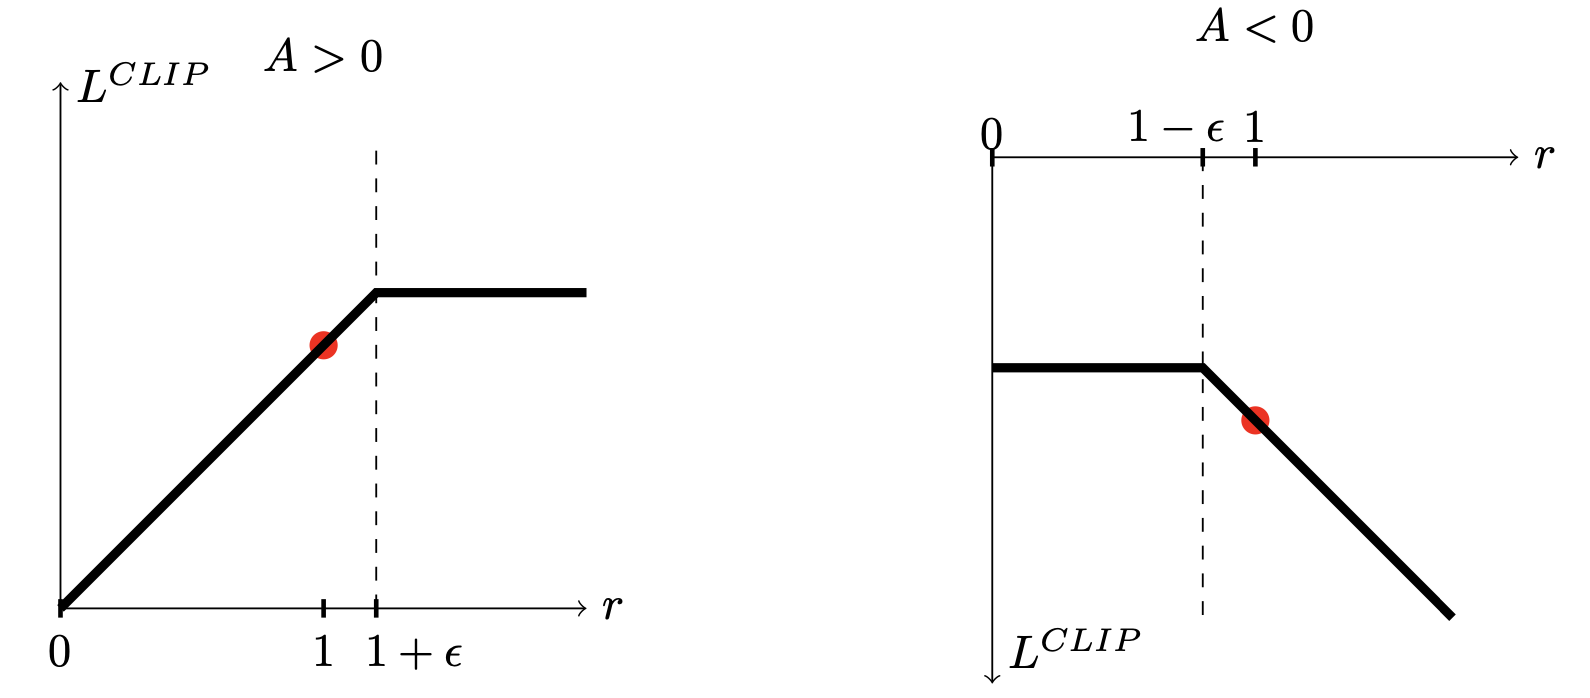
\includegraphics[width=0.5\linewidth]{figures/ppo-clip.png}
    \caption{\emph{PPO w/ clipped objective}. Plots showing $\mathcal{L}^{CLIP}$ as a function of the probability ratio $r$, for positive advantages (left) and negative advantages (right). The red circle on each plot shows the starting point for the optimization, i.e., $r=1$. More detailed explanations \href{https://stackoverflow.com/a/50663200}{here}. Figure taken from \cite{schulman2017proximal}.}
    \label{fig:ppo-clip}
\end{figure}

\subsection{Off-Policy}
Although actor-critic methods such as PPO or A2C/A3C are already re-using a couple recent samples, they are not as sample-efficient as off-policy value-based methods. \emph{Off-policy policy gradient} methods improve this, and make it possible to define better exploration strategies.

In this section, samples are collected with a \emph{behavior policy} $\mu$, typically different from our learned policy $\pi_\theta$.

\paragraph{Off-policy policy gradient theorem}
Given a behavior policy $\mu$ and its stationary distribution $d^\mu(s) = \lim_{t\rightarrow \infty} P(s_t = s \mid \mu)$ (see eq. \ref{eq:stationary-state-distribution}), we can define an \emph{off-policy performance objective} \footnote{
This is slightly different from the on-policy reward that we have been considering so far: $J(\theta) = \E_{\tau \sim \pi_\theta}[R(\tau)] = \E_{s_0 \sim \rho_0}[V^{\pi_\theta}(s_0)]$.
}:

\[
    J_\mu(\theta) = \E_{s_0 \sim \mu}[V^{\pi_\theta}(s_0)]
\]
The off-policy policy gradient can then be expressed as:
\begin{align}
    \nabla_\theta J_\mu(\theta)
    &= \nabla_\theta \E_{s\sim d^\mu} \left[ \sum_a \pi_\theta(a\mid s) Q^{\pi_\theta}(s,a) \right] \nonumber \\
    &= \E_{s\sim d^\mu} \left[ 
        \sum_a \nabla_\theta \pi_\theta(a\mid s) Q^{\pi_\theta}(s,a) + 
        \underbrace{\pi_\theta(a\mid s) \nabla_\theta Q^{\pi_\theta}(s,a)}_{\approx 0}
    \right] \nonumber \\
    &\approx \E_{s,a \sim \mu} \left[
        \frac{\pi_\theta(a\mid s)}{\mu(a\mid s)} Q^{\pi_\theta}(s,a) \nabla_\theta \log \pi_\theta(a\mid s)
    \right]
    \label{eq:off-policy-policy-gradient}
\end{align}

The approximation is necessary since $\nabla_\theta Q^{\pi_\theta}(s,a)$ is typically hard to compute. However, this biased gradient still improves the policy and allows converging to the right solution, at least in the tabular case (off-policy policy gradient theorem, \cite{degris2012off}).

\emph{Note}. Eq. \ref{eq:off-policy-policy-gradient} closely resembles the on-policy gradient (eq. \ref{eq:policy-gradient}), but with an added weight $\frac{\pi_\theta(a\mid s)}{\mu(a\mid s)}$, and using the stationary distribution. 
The \emph{policy gradient theorem} \footnote{Proof can be found \href{https://lilianweng.github.io/lil-log/2018/04/08/policy-gradient-algorithms.html\#policy-gradient-theorem}{here} or \href{https://stanford.edu/~ashlearn/RLForFinanceBook/PolicyGradient.pdf}{here}} actually states that:
\begin{align}
    \nabla_\theta J(\theta)
    &= \E_{s\sim d^{\pi_\theta}} \left[ \sum_a Q^{\pi_\theta}(s,a) \nabla_\theta \pi_\theta(a\mid s) \right]
    \nonumber \\
    &= \E_{s,a\sim \pi_\theta} \left[ Q^{\pi_\theta}(s,a) \nabla_\theta \log \pi_\theta(a\mid s) \right]
\end{align}

\paragraph{Estimating $Q^\pi$ in off-policy}

\emph{Tabular case (discrete action and state spaces)}.
Using a slightly different TD error $\delta_t = r_t + \gamma \E_{a\sim \pi(\dot \mid s_{t+1}}[Q(s_{t+1})] - Q(s_t,a_t)$, we can estimate $Q^\pi$ with TD-0 learning, even if our samples $(s_t, a_t, s_{t+1})$ are not collected with policy $\pi$:
\[
Q(s_t, a_t) \leftarrow Q(s_t, a_t) + \alpha \delta_t
\]

Multi-step learning is harder however, since the next actions $a_{t+k}$ are sampled from the behavior policy $\mu$:
\[
Q(s, a) \leftarrow Q(s, a) + \alpha \E_{s_t,a_t,s_{t+1} \sim \mu, \forall t} \left[ 
    \sum_{t=0}^k \gamma^t \left( \prod_{i=0}^t c_i \right) \left( 
        r_t + \gamma \E_{a_{t+1}\sim \pi} [Q(s_{t+1}, a_{t+1})] - Q(s_t,a_t)
    \right) \mid s_0 = s, a_0 = a
\right]
\]
With $c_i$ a coefficient that can be
\begin{itemize}
    \item $c_i = \lambda$: regular $Q(\lambda)$ algorithm, but biased since we are off-policy, and only converges if $\mu$ and $\pi$ are close
    \item $c_i = \frac{\pi(a_i\mid s_i)}{\mu(a_i\mid s_i)}$: unbiased thanks to importance sampling, but not stable (high variance)
    \item $c_i = \lambda \pi(a_i\mid s_i)$: \emph{Tree Backup} \cite{precup2000eligibility} works even when $\mu$ and $\pi$ are different, but not efficient due to premature “cuts” if $\pi(a_i\mid s_i)$ becomes small.
    \item $c_i = \lambda \min(1, \frac{\pi(a_i\mid s_i)}{\mu(a_i\mid s_i)})$: \emph{Retrace} \cite{munos2016safe} combines the best of both worlds, with controlled variance $c_i \leq \lambda$), no premature “cuts”, and even has guarantees of convergence.
\end{itemize}

\emph{Approximate case (e.g. continuous state space)}.
Here as well we can use the Retrace coefficient $c_i$, but learning $Q_\theta(s,a)$ requires a target value $Q^{ret}$ in order to compute an error (e.g. least square) and a gradient. For each trajectory $\tau$, the target can be defined recursively (starting from the final value $Q^{ret}(s_{T-1}, a_{T-1}) = r_{T-1}$):
\[
Q^{ret}(s_t, a_t) = r_t + \gamma c_{t+1} [Q^{ret}(s_{t+1}, a_{t+1}) - Q_\theta(s_{t+1}, a_{t+1})] + \gamma E_{a\sim \pi} Q_\theta(s_{t+1}, a)
\]

\paragraph{Actor-Critic with Experience Replay (ACER)} \cite{wang2016sample}
Similar to on-policy actor critic methods (e.g. A3C/A2C), learning an estimate of $Q^\pi$ in eq. \ref{eq:off-policy-policy-gradient} can reduce the variance. ACER decomposes $\nabla_\theta J_\mu(\theta)$ into
\begin{align*}
\nabla_\theta J_\mu(\theta) = \E_{s_t\sim \mu} \biggl[
    & \E_{a_t\sim \mu}[
        \min(c, \omega_t(a_t)) Q^\pi(s_t, a_t) \nabla_\theta \log \pi_\theta(a_t\mid s_t)
    ] \\
    & + \E_{a\sim \pi}\left[
        \max\left(0, \frac{\omega_t(a)-c}{\omega_t(a)}\right) Q^\pi(s_t, a) \nabla_\theta \log \pi_\theta(a\mid s_t)
    \right]
\biggr]
\end{align*}

With $c$ a hyper-parameter and $\omega_t(a) = \frac{\pi(a\mid s_t)}{\mu(a\mid s_t)}$ the importance sampling ratio. The left term clips this ratio to bound the variance, the right term ensures that the estimate is unbiased. Using our estimates of $Q^\pi$, and substracting our estimate $V_{\theta_v}$ of $V^\pi$ to further reduce the variance, the gradient estimate becomes:
\begin{align*}
    g_t^\text{acer} = 
    & \min(c, \omega_t(a_t)) (Q^{ret}(s_t, a_t) - V_{\theta_v}(s_t)) \nabla_\theta \log \pi_\theta(a_t\mid s_t) \\
    &+ \E_{a\sim \pi}\left[
        \max\left(0, \frac{\omega_t(a)-c}{\omega_t(a)}\right) 
        (Q_{\theta_v}(s_t, a) - V_{\theta_v}(s_t)) \nabla_\theta \log \pi_\theta(a\mid s_t)
    \right]
\end{align*}

In addition to this, ACER does trust-region updates (like TRPO) but actually considers the gradient $g_{\phi_\theta(s_t)}$ w.r.t. the policy distribution parameters $\phi_\theta(s)$ (e.g. logits or probability vector of discrete actions) instead of the model parameters $\theta$. With $\pi_{\theta_a}$ a smoothly updated average policy, the following optimisation problem is solved: 
\[
    \min_z \frac{1}{2} \mid \mid g_{\phi_\theta(s_t)} - z\mid \mid ^2 \quad \text{s.t.} \quad
    \nabla_{\phi_\theta(s_t)} D_{KL}[
        \pi_{\theta_a}(\cdot \mid s_t) \mid \mid \pi_\theta(\cdot \mid s_t)
    ]^T z \leq \delta
\]
Which has a closed form solution $z^*$. Policy parameters $\theta$ are updated using the gradient $g_\theta = z^* \nabla_\theta \phi_\theta(s_t)$.


\subsection{Continuous Action Spaces}
Previous policy gradients methods can be used with either a discrete or continuous action space (e.g. $\mathcal{A} \in \mathbb{R}^d, \pi(a\mid s) = \mathcal{N}(a; \mu_\theta(s), \Sigma_\theta(s))$). But continuous action spaces actually allow taking the gradient w.r.t. actions $\nabla_a Q_\theta(s,a)$ and deriving specific algorithms.

\paragraph{Deterministic Policy Gradients (DPG/DDPG)} \cite{silver2014deterministic} \cite{lillicrap2015continuous}
In addition to a continuous action space, DPG considers a non-stochastic policy taking actions $a = \mu_\theta(s)$. The on-policy policy gradient becomes:
\begin{equation}
    \nabla_\theta J(\theta) = \E_{s\sim d^{\pi_\theta}} \left[
        \nabla_a Q^{\pi_\theta}(s,a) \Bigr|_{a=\mu_\theta(s)} \nabla_\theta \mu_\theta(s)
    \right]
\label{eq:ddpg-on-policy}
\end{equation}
And critic $Q^{\pi_\theta}$ can be learned with SARSA updates.

In order to add exploration and to be more sample-efficient, an off-policy version is also proposed:
\begin{equation}
    \nabla_\theta J_\beta(\theta) \approx \E_{s\sim d^\beta} \left[
        \nabla_a Q^{\pi_\theta}(s,a) \Bigr|_{a=\mu_\theta(s)} \nabla_\theta \mu_\theta(s)
    \right]
\label{eq:ddpg-off-policy}
\end{equation}
Doing the same approximation as in \ref{eq:off-policy-policy-gradient} (and this time we call $\beta$ the behavior policy). Critic can be learned with Q-learning updates.

DDPG simply implements the off-policy version of DPG with deep neural networks for $Q^\pi$ and $\mu_\theta$, and adding noise to $\mu_\theta$ to construct the exploration policy. Stability is achieved by using tricks from DQN: replay buffer, target networks and soft updates. A couple extensions use additional tricks: 2 value networks $Q^\pi$ like Double DQN (TD3 \cite{fujimoto2018addressing}), Prioritized replay and a distributional critic (D4G \cite{barth2018distributed}).


\paragraph{Policy gradient with an off-policy critic (Q-Prop)} \cite{gu2016q}
While off-policy methods like DDPG are more sample efficient than REINFORCE, the off-policy gradient (eq. \ref{eq:ddpg-off-policy}) is biased and typically less stable (requiring fine hyper-parameter optimization). The Q-Prop algorithm uses an unbiased on-policy gradient (more stable) but reduces the variance (more sample efficient) thanks a control variate $\eta(s_t)$ and an off-policy critic $Q_w$ learned like in DDPG.

\begin{align}
    \nabla_\theta J(\theta) = 
    & \E_{s_t\sim d^\pi, a_t \sim \pi} \underbrace{
        \left[
            \nabla_\theta \log \pi_\theta(a_t\mid s_t) (\hat{A}(s_t,a_t) - \eta(s_t) \overline{A_w}(s_t,a_t))
        \right]
    }_{
        \text{REINFORCE correction term ($\approx 0$ if $Q_w$ is good)}
    }
    \nonumber \\
    & + \E_{s_t\sim d^\pi} \underbrace{
        \left[
            \eta(s_t) \nabla_a Q_w(s_t,a) \Bigr|_{a=\mu_\theta(s_t)} \nabla_\theta \mu_\theta(s_t)
        \right]
    }_{
        \text{On-policy policy gradient with control variate $\eta(s_t)$}
    }
\end{align}

With
\begin{itemize}
    \item $\overline{Q}(s_t,a_t) = Q_w(s_t, \mu_\theta(s_t)) + \nabla_a Q_w(s_t,a) \Bigr|_{a=\mu_\theta(s_t)}(a_t-\mu_\theta(s_t))$ (1st order Taylor approximation)
    \item $\overline{A}(s_t,a_t) = \overline{Q}(s_t,a_t) - \E_{a \sim \pi_\theta}\left[\overline{Q}(s_t,a)\right] = \nabla_a Q_w(s_t, a) \Bigr|_{a=\mu_\theta(s_t)} (a_t-\mu_\theta(s_t))$
    \item $\hat{A}(s_t,a_t)$ estimated with GAE (using $V_w$ learned on-policy)
    \item $\eta(s_t) = 1$ if $\hat{A}(s_t,a_t) \overline{A}(s_t,a_t) > 0$ (i.e. our estimate of $A^\pi$ according to $Q_w$ at least has the same sign than the observed advantage $\hat{A}$), and $\eta(s_t) = 0$ otherwise.
\end{itemize}